\section{Case Studies}

This section presents three case studies on the application of StreetVizor in assisting urban planners to explore and compare human-scale urban forms on the city-, region-, and street-scales.

\begin{figure}[t]
	\centering
	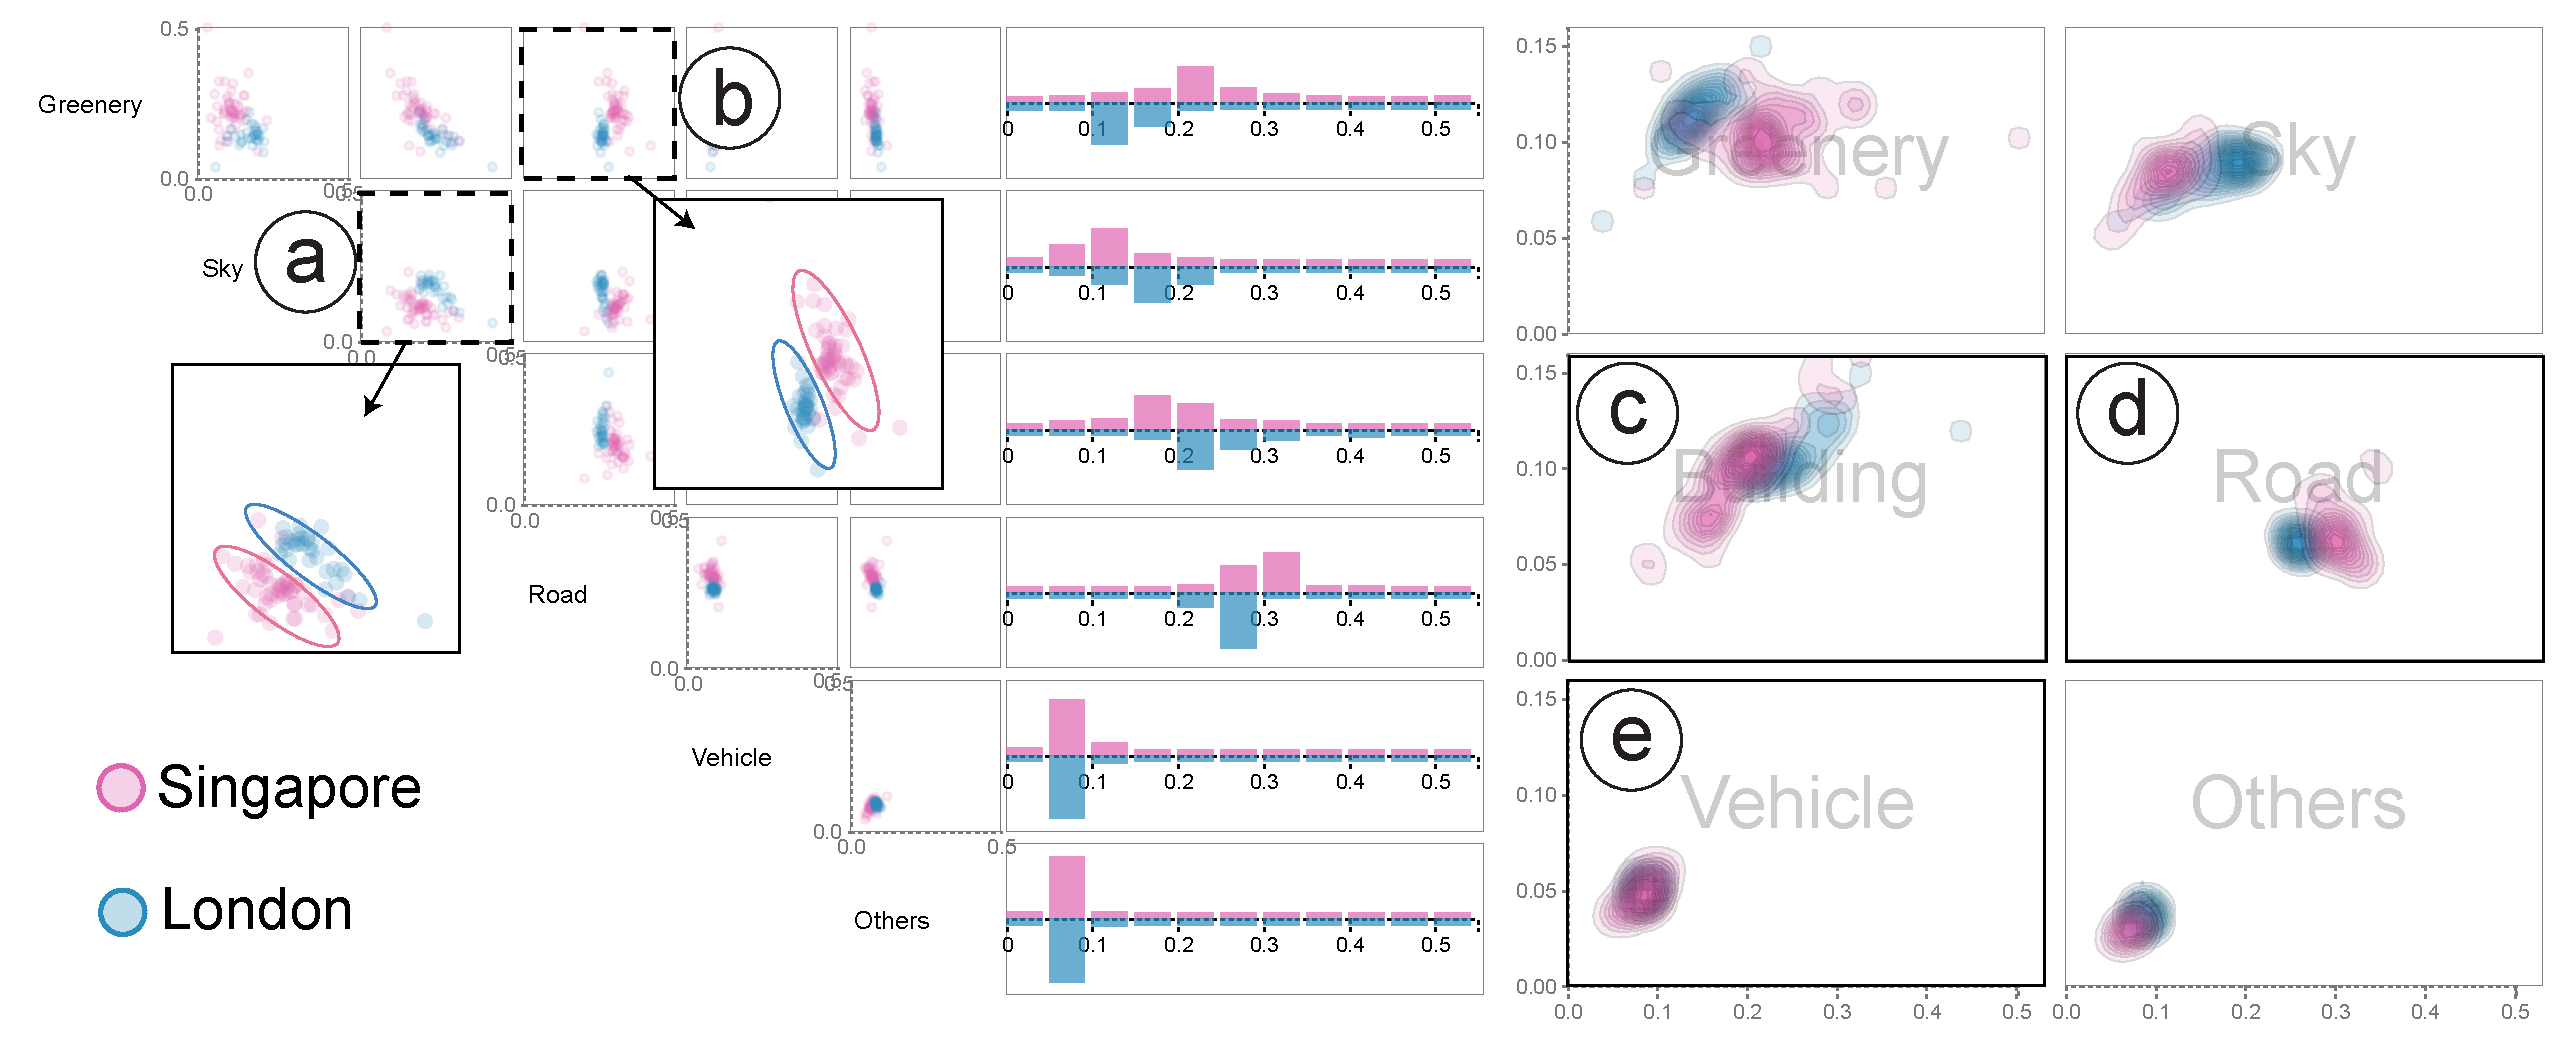
\includegraphics[width=\columnwidth]{figure/streetvizor/fig8_study_1/study_1_statistic}
	\vspace{-7mm}
	\caption{AOI Statistic View in coordination with Fig.~\ref{fig:c1_study_1_spatial} presents quantitative measurements differences of human-scale urban forms in Singapore (red) and Greater London (blue).}
	\label{fig:c1_study_1_statistic}
	\vspace{-1mm}
\end{figure}



%=================================================
\subsection{City-scale Comparison}

\textit{Comparing Spatial Distribution}.
With the AOI Map View, our system allows users to compare spatial distributions of human-scale urban forms in two AOIs (T.1.1).
Fig.~\ref{fig:c1_study_1_spatial} presents a comparison between Singapore (left) and Greater London (right).
As shown in the figure, more orange points surround the highlighted white circle, whereas more green points can be found at marginal areas in Greater London.
This indicates that more buildings are constructed around the City of London, reflecting that this city is more urbanized compared with other areas.
By contrast, Singapore's urban forms are evenly distributed.
More orange points are found in the highlighted downtown and region hubs, and more green points can be found in natural areas.
Our collaborator $SR$ explained the reason for the different spatial distributions of urban forms in Greater London and Singapore: Greater London likely expanded its urbanization from the City of London to surrounding areas, whereas Singapore, as an island city, cannot expand.
% The reason of this difference between Greater London and Singapore may be that Grater London expands its urbanization from City of London to surrounding areas, while Singapore as an island city cannot expand, as explained by our collaborator $SR$.

\vspace*{2mm}
\noindent
\textit{Comparing Quantitative Measurements}.
We can further explore the differences in quantitative measurements with AOI Statistic View (T.2.1 \& T.3.3).
Fig.~\ref{fig:c1_study_1_statistic} shows the AOI Statistic View in coordination with Fig.~\ref{fig:c1_study_1_spatial}.
From the scatterplot matrix, we find that $greenery$ and $building$ features are negatively correlated.
This result is the same as that shown in Fig.~\ref{fig:c1_statistic_view}(d).
Given that $buildings$ are artifacts and $greenery$ is natural, the negative correlation between $building$ and $greenery$ features in all four cities indicates that artifacts increase and natural environments decrease with increasing urbanization.
To improve livability, many urban planners have proposed integrating more natural spaces in street space.
In addition, Fig.~\ref{fig:c1_study_1_statistic}(a) shows that $sky$ and $building$ ratios are higher in London than in Singapore.
By contrast, $greenery$ and $road$ ratios are higher in Singapore than in London (Fig.~\ref{fig:c1_study_1_statistic}(b)).
These findings can also be found from the middle histogram bar charts.
In addition, the diversity views further show some interesting patterns.
For example, $building$ and $road$ diversities are more concentrated in London than those in Singapore, as shown in Fig.~\ref{fig:c1_study_1_statistic}(c) \& (d), and likely resulted from the different standards for building and road construction in the two cities.
$Vehicle$ usage rates are low in both cities, as shown in Fig.~\ref{fig:c1_study_1_statistic}(e).


%=================================================
\subsection{Region-scale Exploration}
\begin{figure}[t]
	\centering
	\includegraphics[width=0.98\columnwidth]{figure/streetvizor/fig9_study_2/region-functionality.png}
	\vspace{-5mm}
	\caption{Top three districts with highest $building$ ratios, while bottom three with highest $greenery$ ratios in Hong Kong.}
	\label{fig:s1_region-funcitonality}
	\vspace{-4mm}
\end{figure}
Given that human-scale urban forms are highly associated with the daily lives of residents, we posit that urban forms could reflect the functionalities of a region.
Study 1 already reveals the negative correlations between $greenery$ and $building$ features, and we hypothesize that these two urban forms can reflect urbanization levels.
To evaluate the hypothesis, we further explore these two features at region-scale (T.1.1).
Using ranking functions, we sort administrative districts in Hong Kong based on these two features.
Fig.~\ref{fig:s1_region-funcitonality} presents an overview of three districts with highest values for each feature.
The top three districts are Yau Tsim Mong, Wan Chai, and Kowloon City.
They are all business centers in Hong Kong, and we find these districts are mostly covered by orange points ($building$). 
By contrast, the bottom three districts contain highest values for $greenery$.
In particular, the greenest district is Southern Island, which is reserved as country parks.
The other two districts are also well-known natural areas in Hong Kong.
 
\begin{figure}[t]
	\centering
	\includegraphics[width=\columnwidth]{figure/streetvizor/fig9_study_2/study_2_2}
	\vspace{-7mm}
	\caption{Region-scale comparison of Tanglin in Singapore with Central Park in New York City.}
	\label{fig:c1_center-park-tanglin}
	\vspace{-1mm}
\end{figure}

In addition to exploring regions with different functionalities, urban planners are also interested in comparing regions with similar functionalities.
Here, we leverage our knowledge of famous regions in two different cities, i.e., Tanglin in Singapore (see the region highlighted as natural in Fig.~\ref{fig:c1_study_1_spatial}) and Central Park in New York City.
Both of these regions are well-known parks.
After selecting these regions, we find that nearly all streets in the two regions are dominated by green points, indicating that both regions contain considerable $greenery$ as intended.
However, we find some differences between these two regions by looking deeper into the Street Statistics View (Fig.~\ref{fig:c1_center-park-tanglin}).
First, through the feature histogram bar charts, we find that Central Park has slightly higher $greenery$ ratios (A1), whereas Tanglin has slightly higher $building$ ratios (A2).
Though these differences are marginal, they reflect that more buildings are present in Tanglin, partially because Singapore tries to maximize land usage for building construction.
In addition, by grouping street views based on street units, we glean more information from the diversity plots.
Here, we first obtain the overview that $greenery$ feature has relatively higher mean values and deviations than the other five features.
We also find some anomalies.
For example, some streets have relatively low mean values but high deviations for $greenery$ in Central Park (B1), whereas certain streets have high sky visibility in Tanglin (B2), and some streets have very high $building$ ratios in both regions (B3).

The results of this study show that human-scale urban forms are correlated with regional functionalities.
Meanwhile, even though two regions may have the same functionalities, street spaces in regions can be different between two cities.
This may reflect the differences in city planning and development strategies between cities.


%=================================================
\subsection{Street-scale Comparison}
Our collaborating domain expert $SR$ is interested in comparing the fine-grained details of two streets (T.1.2).
StreetVizor meets this requirement with Street Explorer.
Here, we select one street from Brooklyn, New York City, and one from Kowloon, Hong Kong.
Both streets are representative streets of each district.

Fig.~\ref{fig:c1_study_3} presents the visual comparison of these two streets.
The map views provide an overview that nearly half of the street views are mostly green ($greenery$), and the other half are mostly orange ($building$) on the street from Brooklyn.
By contrast, the street views in Kowloon are mostly orange ($building$).
We can observe more details by looking at the street view images.
As shown on the top images, more $greenery$ and $sky$ with low $buildings$ are seen in the left two images, whereas the right two images are filled with $building$ and $road$.
The tree map of the leftmost image shows the street view is well balanced with $greenery$, $road$, $building$, and $vehicle$ features.
Notice that the street view is also highlighted in the bottom Street Statistic View.
More details on the quantitative measurements of street views can be observed in the bottom Street Statistic View.
The themeriver plots clearly show differences in feature distributions:
street views in Brooklyn are more mixed with balanced $greenery$, $sky$, $building$, $road$, and $vehicle$ features, whereas street views in Kowloon are mostly filled with $building$ and $road$ features.
The histogram bars in PCP further confirm this observation: most street views in Kowloon have less than 10\% $greenery$ and $sky$.

Though it is well known in the field of urban planning that New York City is well integrated with natural features and that Hong Kong has more high-rise buildings, $SR$ is excited to see our system can present these differences so intuitively.
``Street Explorer can definitely improve our work efficiency,'' $SR$ commented.


\begin{figure}[t]
	\centering
	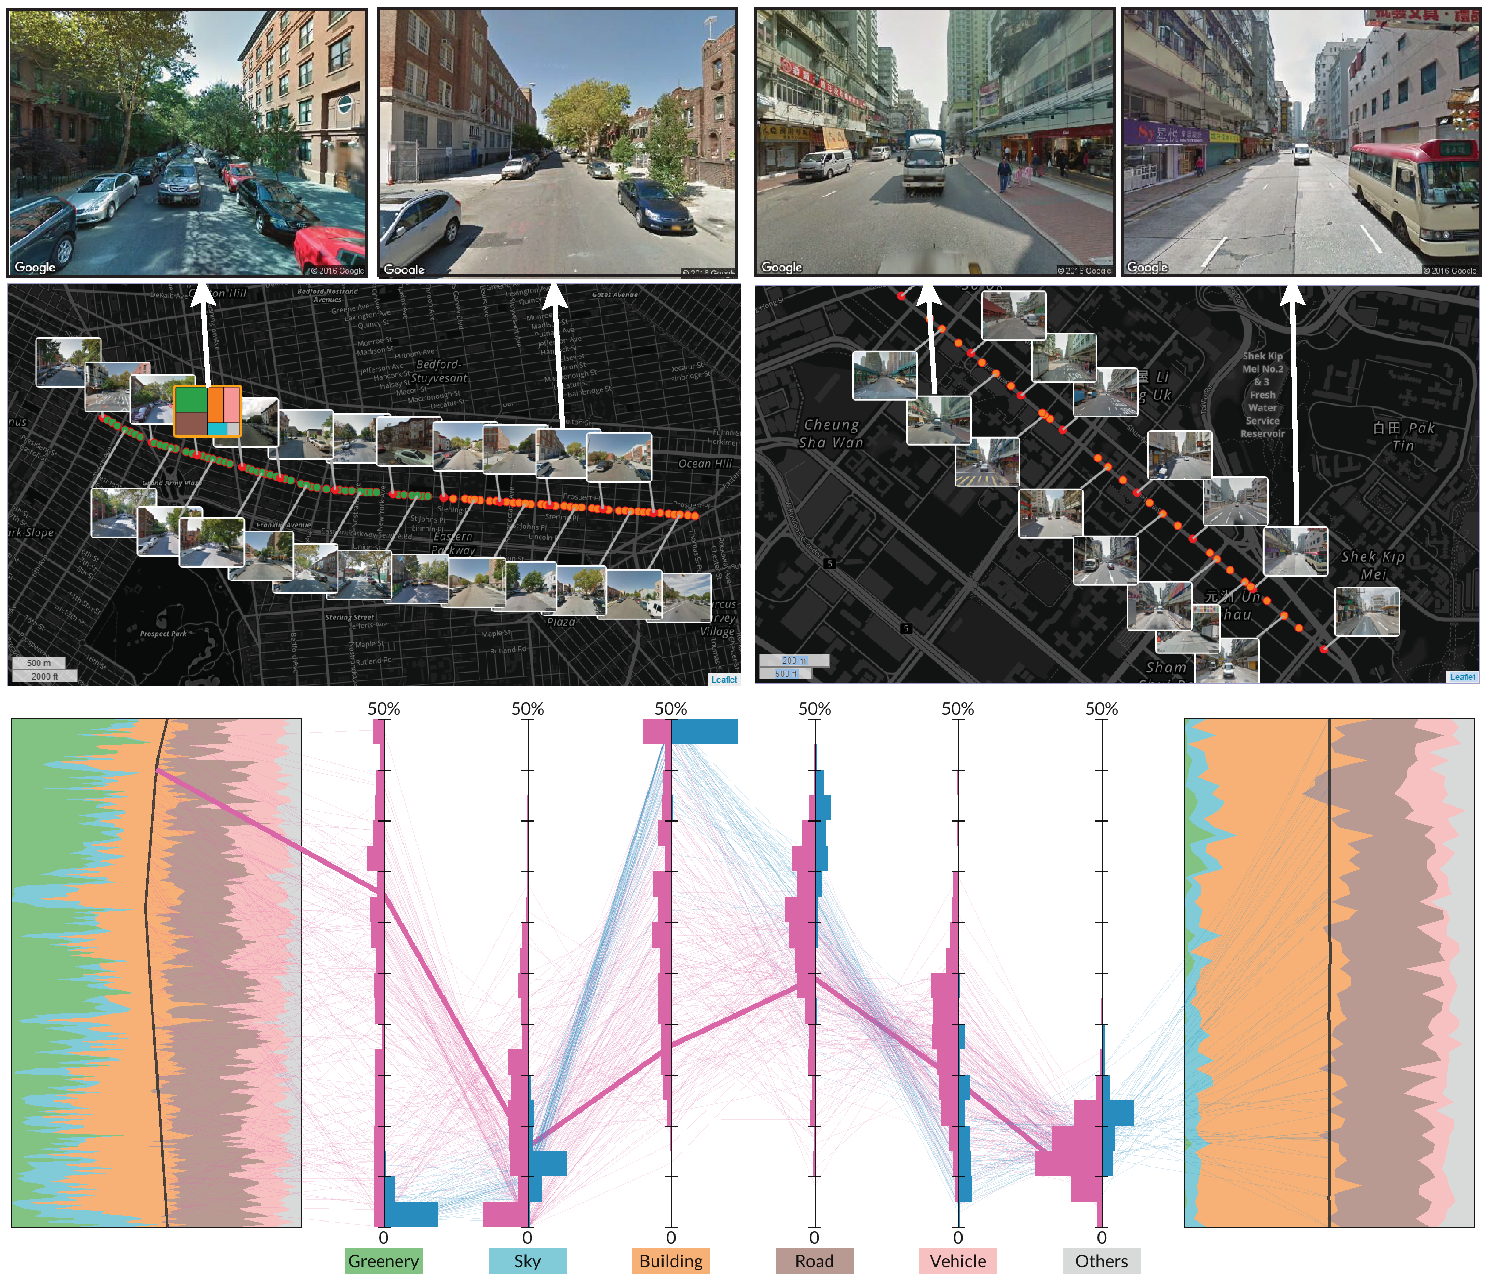
\includegraphics[width=0.95\columnwidth]{figure/streetvizor/fig10_study_3/study_3}
	\vspace{-4mm}
	\caption{Street Explorer compares the differences in human-scale urban forms of two streets in Brooklyn, New York City (left) and Kowloon, Hong Kong (right).
	The left street views contain more balanced features, whereas the right street views are dominated by $building$ and $road$.}
	\label{fig:c1_study_3}
	\vspace{-1mm}
\end{figure}